\documentclass[a4paper]{article}
\usepackage{amsmath}
\usepackage{hyperref}
\usepackage{pgfplots}
\pgfplotsset{compat=1.15}
\usepackage[english]{babel}

\usepackage{listings}
\usepackage{color}

\definecolor{dkgreen}{rgb}{0,0.6,0}
\definecolor{gray}{rgb}{0.5,0.5,0.5}
\definecolor{mauve}{rgb}{0.58,0,0.82}

\lstset{frame=tb,
  language=Java,
  aboveskip=3mm,
  belowskip=3mm,
  showstringspaces=false,
  columns=flexible,
  basicstyle={\small\ttfamily},
  numbers=none,
  numberstyle=\tiny\color{gray},
  keywordstyle=\color{blue},
  commentstyle=\color{dkgreen},
  stringstyle=\color{mauve},
  breaklines=true,
  breakatwhitespace=true,
  tabsize=3
}

\begin{document}
\title{Measurement analysis of speed across multiple methods of grey-scaling}
\author{Niels de Waal (1698041), Jasper Smienk(1700502)}
\maketitle
\newpage

\tableofcontents
\newpage

\section{Target}
With this measurement analysis we want to find out how fast each grey-scaling method is and compare them to each other and the default implementation.

These results can help improve the speed of the facial recognition because converting an image to grey-scale is one of the steps that needs to be done. This step needs to be done for every frame to improve the facial recognition success rates. Having to do the grey-scaling every frame could, over time, add up to a lot of computation. While this time could be of high value in applications where the recognition process needs to be done in real-time.

\section{Hypothesis}
We suspect that of our methods the \textit{decomposition} will be the fastest, as it required very little computation. Followed by \textit{averaging} and lastly \textit{luma}.

We suspect \textit{decomposition} to be the fasted because of the fact that modern cpus have build-in instructions that can take care of the necessary analysis.

We can't say anything about how they will perform against the default implementation, as we don't know how it works.

\section{Method}
For each grey-scaling method, we will run it 10000 times and see how long it took from the start to the end. From this we will calculate the average time it took.

The test will be run twice for each method, once with the facial recognition, and once without.

We will make sure the tests are run on the same laptop and keep an eye out on the temperature to make sure it does not thermal-throttle.

Specifications of the used laptop:
\begin{center}
    \begin{tabular}{ | l | l |}
    \hline
    CPU & Intel i7 8550U \cite{ARK} \\ \hline
    RAM & 16GB DDR4 2400MHz \\ \hline
    OS & Linux 4.15.15-1-ARCH \\ \hline
    \end{tabular}
\end{center}


\newpage
\section{Results}
\subsection{Raw data}
\begin{center}
\begin{tabular}{ |l||r|r| }
\hline
Method & Speed total (ns) & Speed greyscale only (ns) \\
\hline\hline
Default & 6287400 & 457354 \\
\hline
Averaging & 6254653 & 430275 \\
\hline
Luma & 6555633 & 568484 \\
\hline
Decomposition (Max) & 6036561 & 468192 \\
\hline
Decomposition (Min) & 6339750 & 467159 \\
\hline
\end{tabular}
\end{center}

\subsection{Visualized}
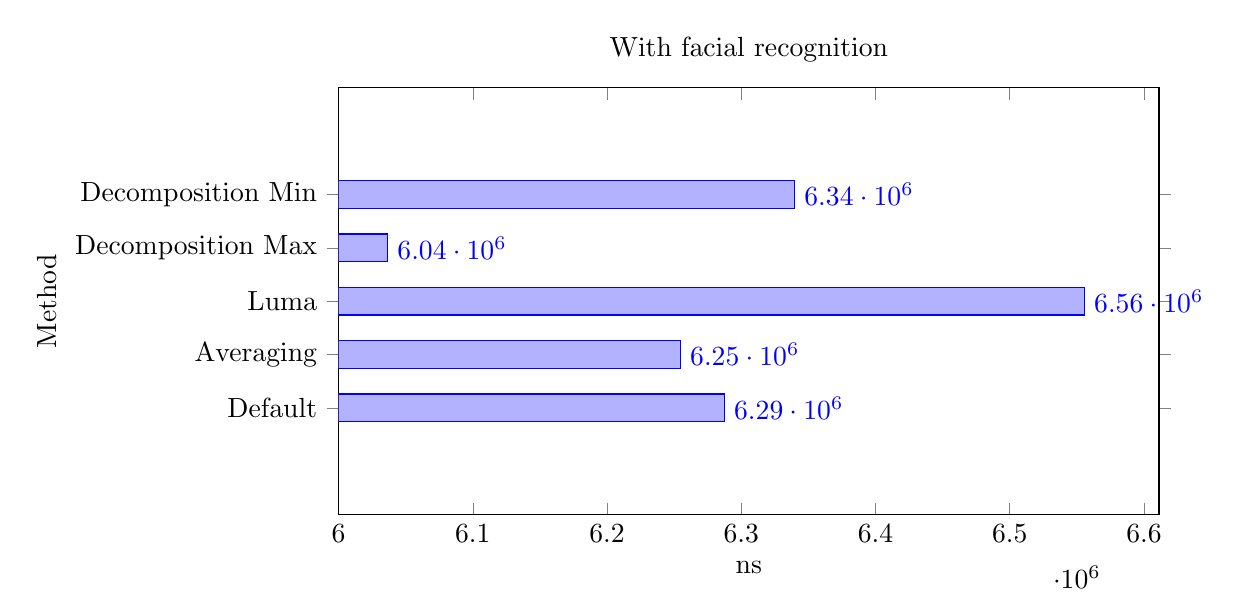
\begin{tikzpicture}
	\begin{axis}[
		title=With facial recognition,
		xbar, xmin=6000000,
		width=12cm,
		height=7cm,
		enlarge y limits=0.5,
		xlabel={ns},
		ylabel={Method},
		symbolic y coords={Default,Averaging,Luma,Decomposition Max,Decomposition Min},
		ytick=data,
		nodes near coords, nodes near coords align={horizontal},
	]
		\addplot coordinates{(6287400,Default) (6254653,Averaging) (6555633,Luma) (6036561,Decomposition Max) (6339750,Decomposition Min)};
	\end{axis}
\end{tikzpicture}
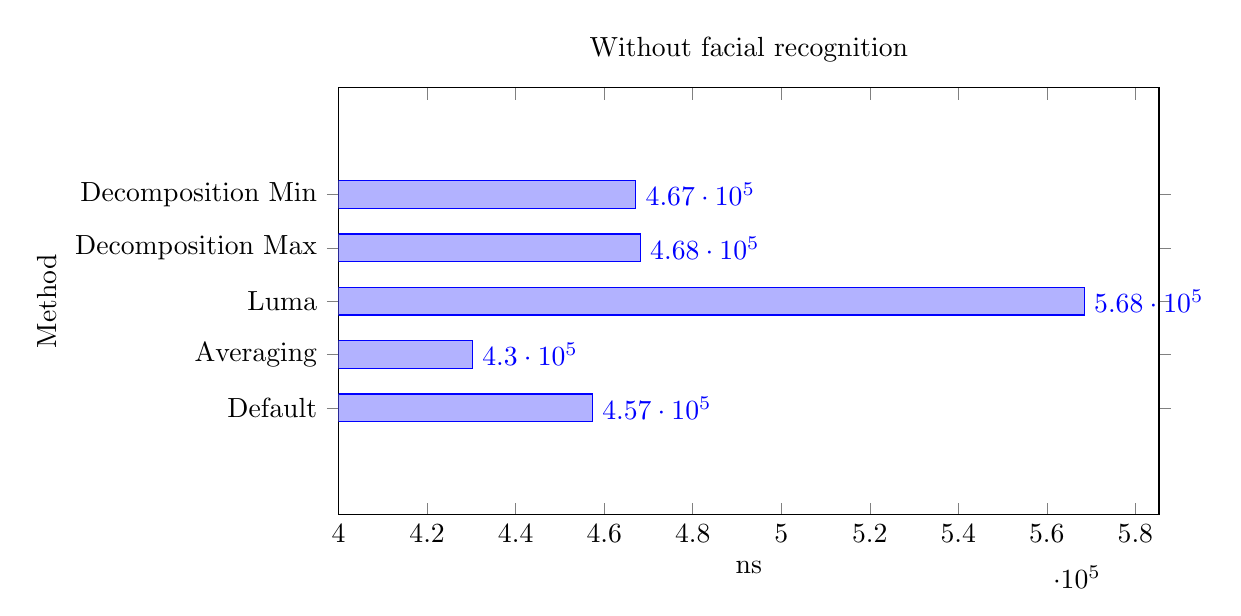
\begin{tikzpicture}
	\begin{axis}[
		title=Without facial recognition,
		xbar, xmin=400000,
		width=12cm,
		height=7cm,
		enlarge y limits=0.5,
		xlabel={ns},
		ylabel={Method},
		symbolic y coords={Default,Averaging,Luma,Decomposition Max,Decomposition Min},
		ytick=data,
		nodes near coords, nodes near coords align={horizontal},
	]
		\addplot coordinates{(457354,Default) (430275,Averaging) (568484,Luma) (468192,Decomposition Max) (467159,Decomposition Min)};
	\end{axis}
\end{tikzpicture}

\section{Processing}
When looking solely at which method is the fastest grey-scale method, \textit{averaging} comes out ahead. Followed by the default method and both \textit{decomposition} methods. At last is \textit{Luma}, which was expected.

We suspect \textit{luma} to be the slowest because of the necessary floating point calculations involved. 

However, \textit{decomposition} max comes out ahead when you also consider the computation time of the facial recognition that follows. Then comes \textit{averaging}, the default and \textit{decomposition} min. \textit{Luma} is last yet again.

\section{Conclusion}
Depending on what you need, different methods are applicable. If you just want the fastest method, use \textit{averaging}. However, if you want to use it with facial recognition, use \textit{decomposition} max.

An other observation is that the facial recognition with the \textit{Luma} method is noticeable slower, even though the grey-scaling is a small part of the whole process. This means that even though \textit{Luma} makes the (subjectively) best looking images for the human eye, they make the facial recognition slower.

\section{Evaluation}
\subsection{What went well}
The project was a very cooperative experience for both parties involved. This cooperation went very well, everyone had their tasks and did them with equal amount of dedication. This made the project an overall pleasant experience.
\subsection{What went wrong}
We both had a vigorous start with the project, however it turned out to be very hard to keep up this speed. Eventually we started to have to divide our time to other projects that required our attention at the time. This made it so we had to do a lot of work near the deadline.

Also the original plan was to use OpenCL and SIMD for parallelism. Because of the state of the relevant tools, this turned out to be quite a bit harder than was originally thought.
\subsection{What could be done differently}
A better research on the more ambitious subjects should be done in order to avoid unnecessary delays.

\section{Additional information}
In this section there will be additional information about the system where the tests where run on.
\subsection{LSCPU}
\begin{lstlisting}[language=bash]
	Architecture:        x86_64
	CPU op-mode(s):      32-bit, 64-bit
	Byte Order:          Little Endian
	CPU(s):              8
	On-line CPU(s) list: 0-7
	Thread(s) per core:  2
	Core(s) per socket:  4
	Socket(s):           1
	NUMA node(s):        1
	Vendor ID:           GenuineIntel
	CPU family:          6
	Model:               142
	Model name:          Intel(R) Core(TM) i7-8550U CPU @ 1.80GHz
	Stepping:            10
	CPU MHz:             1772.800
	CPU max MHz:         4000.0000
	CPU min MHz:         400.0000
	BogoMIPS:            3984.00
	Virtualization:      VT-x
	L1d cache:           32K
	L1i cache:           32K
	L2 cache:            256K
	L3 cache:            8192K
	NUMA node0 CPU(s):   0-7
	Flags:               fpu vme de pse tsc msr pae mce cx8 apic sep mtrr pge mca cmov pat pse36 clflush dts acpi mmx fxsr sse sse2 ss ht tm pbe syscall nx pdpe1gb rdtscp lm constant_tsc art arch_perfmon pebs bts rep_good nopl xtopology nonstop_tsc cpuid aperfmperf tsc_known_freq pni pclmulqdq dtes64 monitor ds_cpl vmx est tm2 ssse3 sdbg fma cx16 xtpr pdcm pcid sse4_1 sse4_2 x2apic movbe popcnt tsc_deadline_timer aes xsave avx f16c rdrand lahf_lm abm 3dnowprefetch cpuid_fault epb invpcid_single pti tpr_shadow vnmi flexpriority ept vpid fsgsbase tsc_adjust bmi1 avx2 smep bmi2 erms invpcid mpx rdseed adx smap clflushopt intel_pt xsaveopt xsavec xgetbv1 xsaves ibpb ibrs stibp dtherm ida arat pln pts hwp hwp_notify hwp_act_window hwp_epp
\end{lstlisting}
\begin{thebibliography}{9}

\bibitem {ARK}
	Intel
	Ark product specifications
	\url{https://ark.intel.com/products/122589/Intel-Core-i7-8550U-Processor-8M-Cache-up-to-4_00-GHz}
	
\end{thebibliography}
\end{document}
